\section{MILP Formulations}
\label{sec:ILP}

In this section, we state and explain MILP formulations of the SMT problem.
A basic element of every MIP formulation for SMT is a set of constraints modelling a Steiner tree.
We investigate two such Steiner tree models with variables of up to 3 node indices and compare SMT models based on them.
Both models are subsequently strengthened by valid inequalities.
Variables with 4 node indices and associated constraints further extend the models.
Valid inequalities added to the extended models result in the strongest known SMT formulations.

\subsection{Formulation based on broadcast trees}

The first model extends the SBT formulation introduced in \cite{Haugland12Dual} by the Steiner nodes in order to formulate the multicast version of the problem \cite{ivanova16isco}.

\subsubsection{Underlying Steiner tree formulation [X0]}

Following \cite{Haugland12Dual}, define the binary variables
\newline\newline
$y_{ij}=
\begin{cases}
    1 & \text{if edge $\{i,j\} \in E$ is in the solution},\\
    0 & \text{otherwise},
  \end{cases}$
\newline\newline
$X^{s}_{ij}=
\begin{cases}
    1 & \text{if arc $(i,j) \in A$ is on a path from $s\in D$},\\
    0 & \text{otherwise}.
  \end{cases}$
\newline\newline
The following constraints imply that $G_y$ is a Steiner tree spanning $D$.
The minimum Steiner tree is formulated as
%%%%%%%%%%%%%%%%%%%%%%%%%%%%%%%%%%%%%%%
%                                     % 
%     STEINER TREE MODEL X0           %
%            (1a) - (1h)              %
%                                     %
%%%%%%%%%%%%%%%%%%%%%%%%%%%%%%%%%%%%%%%
\begin{subequations}\label{mod:x0}
\begin{align}
\label{con:dd:arrowFromDest} \sum\limits_{j\in V_i}X^s_{ji} & = 1 & i,s\in D,i\neq s,\\
\label{con:dd:arrowFromNonDestB} \sum\limits_{j\in V_{i}}X^s_{ji} & \leq 1 & i\in V \setminus D, s\in D,\\
\label{con:dd:arrowFromNonDestA} X^s_{ij} & \leq \sum\limits_{k\in V_{i}\setminus \{j\}}X^s_{ki} & i\in V \setminus D,(i,j)\in A, s\in D,\\
\label{con:dd:oneDir} X^s_{ij} + X^s_{ji} & = y_{ij} & \{i,j\}\in E, s\in D,\\
\label{con:dd:startInSource} X^s_{js} & = 0 &  s\in D, (j,s)\in A,&\\
\label{con:dd:vardim}y \in \{0,1\}^{E}, X & \in \{0,1\}^{A\times D}.
\end{align}~
\end{subequations}

Let $(X,y)$ be an optimal solution to X0.
Then for each $s\in D$, $X^s\in \{0,1\}^{A}$ induces a Steiner arborescence $G_{X^s}$ rooted at source $s$.
From $y\in \{0,1\}^E$ we obtain the resulting (undirected) Steiner tree $G_{y}$ modeled by (\ref{con:dd:arrowFromDest})-(\ref{con:dd:startInSource}).
Constraint (\ref{con:dd:arrowFromDest}) ensures that there is exactly one predecessor $j\in V$ of a destination $i\in D$ in $G_{X^s}$.
Analogously, (\ref{con:dd:arrowFromNonDestB}) covers the case when $i \in V\setminus D$: for every source $s$, there is at most one inbound arc to a non-destination $i$.
If there is an arc $(i,j)$ in $G_{X^s}$ for a non-destination $i$, there must also be an arc $(k,i)$ such that $k\neq j$.
This is enforced by (\ref{con:dd:arrowFromNonDestA}).
Expression (\ref{con:dd:oneDir}) ensures that an edge $\{i,j\}$ is part of the resulting Steiner tree $G_{y}$ if and only if for every $s\in D$, either $(i,j)$ or $(j,i)$ is in $G_{X^s}$.
The next constraint (\ref{con:dd:startInSource}) expresses that $s$ does not have any inbound arc in $G_{X^s}$, which implies non-existence of a directed cycle containing $s$.
%Note that assuming there is no outgoing arc from a non-destination $j$, (\ref{con:dd:arrowFromNonDestA}) does not prevent $j$ from being a leaf in $G_{\mathbf{X^s}}$.
%Even though such solutions do not change the objective value of an integral solution, a Steiner tree by definition does not contain Steiner leaves.
%We therefore disallow them by adding constraint (\ref{con:dd:extraCon}) reducing the set of feasible solutions.

Conversely, for any Steiner tree $T$ spanning $D$, there exists a pair $(X,y)$ satisfying the constraints such that $G_y=T$. 

\subsubsection{SMT model [X1]}

A Steiner arborescence for $G_{X^s}$ can be regarded as a broadcast arborescence describing how a signal initiated in $s$ is routed towards remaining destinations. 
Then, it can also be understood that $X_{ij}^s=1$ if and only if arc $(i,j)$ is used to transmit a signal from $s\in D$.
With this notion, consider variables
\newline\newline
$\pi^s_{ij}=
\begin{cases}
    1 & \text{if node $i \in V$ uses power $p_{ij}$ to transmit a message from $s\in D$},\\
    0 & \text{otherwise},
  \end{cases}$
\newline\newline
leading to the following formulation X1 of SMT:

%%%%%%%%%%%%%%%%%%%%%%%%%%%%%%%%%%%%%%%
%                                     % 
%             MODEL X1                %
%            (1a) - (1k)              %
%                                     %
%%%%%%%%%%%%%%%%%%%%%%%%%%%%%%%%%%%%%%%
\begin{subequations}[resume]\label{eq:smt-x2}
\begin{align}
\label{objective:mf} \makebox[0pt][l]{$\displaystyle{} \min \sum\limits_{(i,j) \in A} \sum\limits_{s \in D} p_{ij} \pi^s_{ij} $}\\
\notag\text{s.t.}\\
\notag(\ref{con:dd:arrowFromDest}) &- (\ref{con:dd:vardim})\\
\label{con:dd:yvar} X^s_{ij} & \leq \sum\limits_{k\in V_i:p_{ik}\geq p_{ij}}\pi^s_{ik} & s\in D, (i,j)\in A,\\
\label{con:dd:vardimy} \pi & \in \{0,1\}^{A\times D}.
\end{align}~
\end{subequations}

This model is a slightly modified version of the SMT model introduced in \cite{ivanova16isco}, which contains a constraint disallowing non-destination leaves and a weaker version of constraint (\ref{con:dd:arrowFromNonDestA}).
By (\ref{con:dd:yvar}), we define a relation between $X$-variables and $\pi$-variables used in the objective function.
Whenever the arc $(i,j)$ is used for transmission of a message from $s\in D$, the power assigned to node $i$ must be at least $p_{ij}$.
In an optimal solution $(X,y,\pi)$ to X1, $\pi^s\in \{0,1\}^{A}$ describes links determining the power levels used by nodes when relaying a message originated in $s$.
The graph induced by $\pi^s$ is  a subgraph of the tree induced by $X^s$, and is not necessarily connected.

\subsubsection{Valid inequalities [X2]}

It is possible to strengthen X1 by adding valid inequalities
%%%%%%%%%%%%%%%%%%%%%%%%%%%%%%%%%%%%%%%
%                                     % 
%             MODEL X1VI              %
%            (1a) - (1k)              %
%                                     %
%%%%%%%%%%%%%%%%%%%%%%%%%%%%%%%%%%%%%%%
\begin{subequations}[resume]
\begin{align}
\label{con:dd:extraCon} \sum\limits_{j\in V_{i}}X^s_{ji} & \leq \sum\limits_{j\in V_{i}}X^s_{ij}  & 	i\in V\setminus D, s\in D,\\
\label{con:vi:Y1} \sum\limits_{j\in V_s}  \pi^{s}_{sj} & =1 & s\in D,\\
\label{con:vi:sumYImpSumX} \sum\limits_{j\in V_i\setminus\{s\} }\pi^{s}_{ij} & \geq \sum\limits_{j\in V_i}  X^{s}_{ji} & i\in V\setminus D, s\in D.
\end{align}
\end{subequations}
Constraint (\ref{con:dd:extraCon}) ensures that $G_{X^s}$, and also any feasible solution, does not contain Steiner nodes as leaves, i.e., a signal never disappears in a non-destination.
%Even though the presence of such leaves does not increase the objective value of an integral solution, it is desirable to eliminate them, because by definition, a Steiner tree does not contain non-destination leaves.
Inequality (\ref{con:vi:Y1}) says that there has to be exactly one neighbour $j\in V$ of $s\in D$, such that $s$ uses the power $p_{sj}$ in order to transmit its own signal.
As (\ref{con:vi:sumYImpSumX}) states, if a non-destination $i$ receives a signal from $s$, then there is a node $j\in V_i\setminus\{s\}$ to which the signal is forwarded requiring power $p_{ij}$ assigned to node $i$.
Index $s$ is excluded from the summation set on the left of (\ref{con:vi:sumYImpSumX}), because (\ref{con:dd:startInSource}) implies that $\pi_{is}^s=0$ is feasible, and $p_{is}\geq 0$ implies that it is optimal in X2. 

\subsubsection{Point to point extension [X3]}
\label{sec:smtx2}

This section introduces variables describing an arc on a path between two destinations, and shows how additional constraints can strengthen model X2.

Consider a directed path from $s\in D$ to $t\in D$.
For this purpose, let $S=\{(s,t)\in D\times D, s\neq t\}$ be the set of ordered pairs of distinct destinations.
In order to model the connectivity requirements, we introduce variables
\newline\newline
$x_{ij}^{st}=
\begin{cases}
    1 & \text{if arc $(i,j) \in A$ lies on a path from $s$ to $t$, $(s,t)\in S$},\\
    0 & \text{otherwise}.
\end{cases}$
\newline\newline

Model X2 can be strengthened by constraints concerning the newly introduced variables, which yields model X3: 
\newline
\newline
%%%%%%%%%%%%%%%%%%%%%%%%%%%%%%%%%%%%%%%
%                                     % 
%             MODEL X2                %
%   (1a) - (1k) and (2b) - (2f)       %
%                                     %
%%%%%%%%%%%%%%%%%%%%%%%%%%%%%%%%%%%%%%%
\begin{subequations}[resume]\label{eq:smt-x2}
\begin{align}
\notag\makebox[0pt][l]{$\displaystyle{} \min \sum\limits_{(i,j) \in A} \sum\limits_{s \in D} p_{ij} \pi^s_{ij} $}\\
\text{s.t.} \notag \\
(\ref{con:dd:arrowFromDest}) - (\ref{con:dd:vardim}) &\text{ and }(\ref{con:dd:yvar}) - (\ref{con:vi:sumYImpSumX}) \notag\\
\label{con:mf:flowNormal} \sum\limits_{\substack{ j\in V_i}}x^{st}_{ij}-\sum\limits_{\substack{j\in V_i }}x^{st}_{ji} & = 0 & (s,t)\in S, i\in V\setminus\{s,t\},\\
%\label{con:mf:flowDest} \sum\limits_{\substack{ j\in V_t }}x^{st}_{tj}-\sum\limits_{\substack{j\in V_t}}x^{st}_{jt}    & = -1  & (s,t)\in S,\\
\label{con:mf:flowDest} \sum\limits_{\substack{j\in V_t}}x^{st}_{jt}    & = 1  & (s,t)\in S,\\
\label{con:mf:fcap} x^{st}_{ij} &\leq X^{s}_{ij}& (i,j)\in A, (s,t)\in S,\\
\label{con:mf:fsym} x^{st}_{ij} &=  x^{ts}_{ji}& (i,j)\in A, (s,t)\in S,\\ 
%\label{con:vi:f2dest}  x^{st_1}_{ij}-x^{st_2}_{ij}+x^{t_1t_2}_{ij} & \geq 0 & (i,j) \in A,\\
%\notag && (s,t_1),(s,t_2),(t_1,t_2)\in S,\\
%\label{con:vi:xImpSumF} X^{s}_{ij} & \leq \sum\limits_{t\in D_s}  x^{st}_{ij} & (i,j)\in A, s\in D, \\
\label{con:vi:sumFImpSumY} \sum\limits_{k\in V_j, p_{jk}\geq p_{ji}}x^{st}_{jk} & \leq \sum\limits_{k\in V_j, p_{jk}\geq p_{ji}}  \pi^{s}_{jk} & i,j\in V, (s,t)\in S,\\
\label{con:mf:xydim} x&\in\{0,1\}^{A\times S}. 
\end{align}~
\end{subequations}

The flow conservation constraints (\ref{con:mf:flowNormal})-(\ref{con:mf:flowDest}) guarantee that for each $(s,t)\in S$, there exists a directed path from $s$ to $t$.
Next, constraint (\ref{con:mf:fcap}) expresses the obvious relation between $X$ and $x$, that if an arc $(i,j)$ lies on a path from $s$ to $t$, then this arc is also on a path from $s$.
The flow symmetry (\ref{con:mf:fsym}) states that arc $(i,j)$ lies on a path from $s$ to $t$ if and only if arc $(j,i)$ lies on a path from $t$ to $s$.

In terms of broadcast trees, we can say that $x_{ij}^{st}=1$ if and only if $(i,j)$ carries a signal initiated in $s$ and directed to $t$.
Consider nodes $i,j\in V$ and a pair of destinations $(s,t)$.
If a message from $s$ to $t$ is sent through $(j,k)$ such that $p_{jk}\geq p_{ji}$, then the message from $s$ must be relayed by $j$ using power level at least $p_{ji}$.
This is expressed by valid inequality (\ref{con:vi:sumFImpSumY}).

\subsection{Formulation based on network flows}

There are many formulations for the Steiner minimum tree problem that can serve as a basis for modelling SMT.
We consider the multi-commodity network flow based model studied in \cite{Polzin}, where the authors use abbreviation $P_{F}$.
The model assumes a given destination $s_0\in D$ that plays the role of a unique source.
To simplify the notation, let $D_0= D_{s_0}$.

\subsubsection{Underlying Steiner tree formulation [F0]}

The model F0 of a Steiner tree contains variables
%
\newline\newline
  $F^{t}_{ij}=
\begin{cases}
    1 & \text{if arc $(i,j) \in A$ lies on a path from $s_0$ to $t\in D_0$},\\
    0 & \text{otherwise},
\end{cases}$
\newline\newline
  $g_{ij}=
\begin{cases}
    1 & \text{if arc $(i,j) \in A$ is a part of the solution},\\
    0 & \text{otherwise},
\end{cases}$
\newline\newline
%
and is formulated as
%%%%%%%%%%%%%%%%%%%%%%%%%%%%%%%%%%%%%%%
%                                     % 
%     MIN. STEINER ARBORESCENCE F0    %
%            (1a) - (1h)              %
%                                     %
%%%%%%%%%%%%%%%%%%%%%%%%%%%%%%%%%%%%%%%
\begin{subequations}
\begin{align}
%\makebox[0pt][l]{$\displaystyle{}\min \sum\limits_{(i,j) \in A} p_{ij} g_{ij} $}  \\ \notag
%\text{s.t.} && \\
\label{con:pf1:xfrel} F^{t}_{ij} & \leq g_{ij} & t\in D_0, (i,j)\in A, \\
\label{con:pf1:flow} \sum\limits_{\substack{ j \in V_i }}F^{t}_{ji}-\sum\limits_{\substack{j\in V_i}}F^{t}_{ij} &= 
  \begin{cases}
    1 & t\in D_0, t = i,\\
    0 & t\in D_0, i\in V\setminus \{s_0, t\},
  \end{cases}\\
%\label{con:pf1:yvar} g_{ij} - F^t_{ij}+F^t_{ji} & \leq \sum\limits_{\substack{k\in V: \\ p_{ik}\geq p_{ij}}}\pi^t_{ik}  & t\in D_0, (i,j)\in A,\\
%\label{con:pf1:yvar0} g_{ij} & \leq \sum\limits_{\substack{k\in V: \\ p_{ik}\geq p_{ij}}}\pi^0_{ik}   &  (i,j)\in A,\\
%\label{con:pf1:B}  \sum_{j\in V_i}g_{ji}&\leq 1 & i\in V\setminus D,\\
%\label{con:pf1:noflowFromT} F_{ti}^t&=0 & t\in D_0, i\in V_t,\\
%\label{con:pf1:fitt=xit} F_{it}^t&=g_{it} & t\in D_0, i\in V_t,\\
%\label{con:pf1:xi0=0} g_{i0}&=0 & i\in V_0,\\
\label{con:pf1:dim}g \in \{0,1\}^{A},F&\in\{0,1\}^{A \times D_0}.
%\label{con:pf1:dimy} y&\in \{0,1\}^{A\times D}.
\end{align}~
\end{subequations}

The $g$-variables inducing the resulting tree correspond to arcs, whereas analogous $y$-variables in X0 correspond to edges.
Hence, an optimal solution to X0 is an undirected tree, and an optimal solution to F0 is an arborescence rooted at $s_0$.
The vector $F^t$ defines a directed path from $s_0$ to $t\in D$ in the arborescence.
Constraints (\ref{con:pf1:xfrel})-(\ref{con:pf1:flow}) together with (\ref{con:pf1:dim}) imply that $g$ induces an arborescence spanning $D$ with node $s_0$ as the root.

We aim to create an SMT model F1 based on F0.
For this purpose, it is necessary to find a way to represent the constraint (\ref{con:dd:yvar}) in the F1 space.
The $\pi$-variables from X1 have to be used in F1, because they appear in the objective function which remains unchanged.
%

%By considering the role of individual sets of variables in both models, the $x$-variables used in X1 are expressed by the variables used in F0 as
%
%\begin{align}
%\label{eq:tr:xijsB}
%\begin{aligned}
%X^s_{ij}&=g_{ij}(1-F^{s}_{ij})(1-F^{s}_{ji})+g_{ji}F^{s}_{ji}=\\
%	&=g_{ij}-F^s_{ij} + F^{s}_{ji} \\
%X^0_{ij} &= g_{ij}
%\end{aligned}
%&&
%\begin{aligned}
%\\
%(i,j)\in A, s\in D_0,\\
%(i,j)\in A.
%\end{aligned}
%\end{align}

\subsubsection{SMT model [F1]}

The model F1 for Problem \ref{def:problem} based on the minimum Steiner arborescence model F0 is constructed as follows: 
%%%%%%%%%%%%%%%%%%%%%%%%%%%%%%%%%%%%%%%
%                                     % 
%             MODEL F1                %
%            (4a) - (4k)              %
%                                     %
%%%%%%%%%%%%%%%%%%%%%%%%%%%%%%%%%%%%%%%
\begin{subequations}[resume]
\begin{align}
\notag\min & \sum\limits_{(i,j) \in A} \sum\limits_{s \in D} p_{ij} \pi^s_{ij}\\ 
\notag\text{s.t.} && \\
\notag(\ref{con:pf1:xfrel}) - (\ref{con:pf1:dim})\\
\label{con:pf1:yvar} g_{ij} - F^t_{ij}+F^t_{ji} & \leq \sum\limits_{\substack{k\in V: \\ p_{ik}\geq p_{ij}}}\pi^t_{ik}  & t\in D_0, (i,j)\in A,\\
\label{con:pf1:yvar0} g_{ij} & \leq \sum\limits_{\substack{k\in V: \\ p_{ik}\geq p_{ij}}}\pi^0_{ik}   &  (i,j)\in A,\\
\label{con:pf1:B}  \sum_{j\in V_i}g_{ji}&\leq 1 & i\in V\setminus D,\\
\label{con:pf1:noflowFromT} F_{ti}^t&=0 & t\in D_0, i\in V_t,\\
\label{con:pf1:fitt=xit} F_{it}^t&=g_{it} & t\in D_0, i\in V_t,\\
\label{con:pf1:xi0=0} g_{i0}&=0 & i\in V_0,\\
\label{con:pf1:dimy} y&\in \{0,1\}^{A\times D}.
\end{align}~
\end{subequations}

Constraints (\ref{con:pf1:yvar}) and (\ref{con:pf1:yvar0}) have the same purpose as (\ref{con:dd:yvar}), and are expressed in F1 space. % using transformations (\ref{eq:tr:xijsB}).
Note that the $\pi$-variables determining power levels are defined for all destinations in $D$, while in the model F1 \cite{Polzin} of the minimum Steiner tree problem, the $F$-variables are defined only for destinations in $D_0$.
For this reason, $\pi_{ij}^0$ is treated separately in (\ref{con:pf1:yvar0}).
%This inconsistency is resolved by adding (\ref{con:pf1:yvar0}), which relates the $\pi^0$-variables with $x$-variables. This is equivalent to extending the the domain of the $f$-variables and fixing the newly introduced variables to zero. 

By (\ref{con:pf1:B}) we prevent a non-destination from having multiple entering arcs.
This is not needed in the minimum Steiner tree problem formulation, because the objective function causes that such solutions are filtered out by optimality.
The necessity of this constraint in SMT is demonstrated in Fig. \ref{fig:BProof}.
%The optimal solution with objective value 25156 to the depicted instance obtained by solving SMT-X1 is shown in Fig. \ref{fig:BorigSMT}.
%The solution in Fig \ref{fig:Bpf2} yielded by solving SMT-F1 without the constraint (\ref{con:pf1:B}) has objective value 25148, but is not a feasible solution to Problem \ref{def:problem}, because of the cycle $(g,h,i,d,g)$.
%The non-existence of such a cycle in a solution given by model X1 is ensured by constraints (\ref{con:dd:arrowFromDest}), (\ref{con:dd:arrowFromNonDestB}) and (\ref{con:dd:oneDir}).
%A detailed proof of this claim can be found in \cite{ivanova16isco}.
%A transmission commenced in node $c$ is sent via arc $(g,f)$.
%As a consequence of the link between $g$ and $d$ in Fig. \ref{fig:Bpf2}, the node $d$ also receives the message.
%This link is absent in Fig. \ref{fig:BorigSMT}, and so $i$ has to relay the signal using arc $(i,d)$, causing the higher total objective value.
Similarly, the obviously valid inequalities (\ref{con:pf1:noflowFromT})-(\ref{con:pf1:fitt=xit}) are not necessary in the minimum Steiner tree formulation, but have to be included in the formulation of SMT, because they  disallow nodes in $D_0$ to have multiple entering arcs.
The same restriction has to be imposed on $s_0$ by including (\ref{con:pf1:xi0=0}).
%%%%%%%%%%%%%%%%%%%%%%%%%%%%%%%%%%%%%%%%%%%%%%%%%%%%%%
%      Figure 2                                      %
%    explaining why some constraints are necessary   %
%%%%%%%%%%%%%%%%%%%%%%%%%%%%%%%%%%%%%%%%%%%%%%%%%%%%%%
\begin{figure}[!htb]
    \centering
    \begin{subfigure}[b]{0.4\textwidth}
        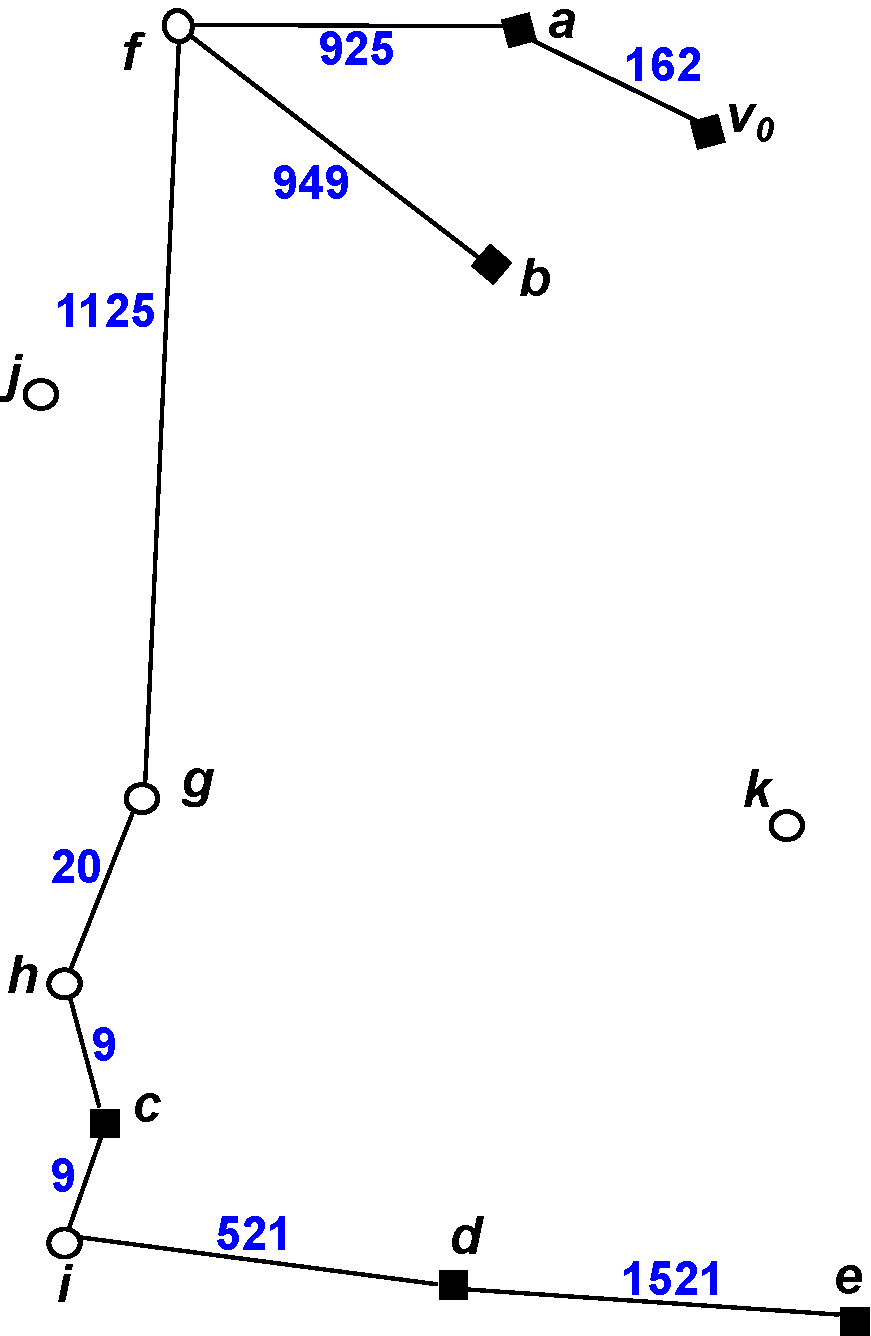
\includegraphics[width=\textwidth]{conBNec}
        \caption{Optimal solution obtained by X1. The $y$-variables inducing the resulting tree in this model represent undirected edges. The objective value of this tree is 25156.\newline~}
        \label{fig:BorigSMT}
    \end{subfigure}
    \hfill
% a blank line to force the subfigure onto a new line
    \begin{subfigure}[b]{0.4\textwidth}
        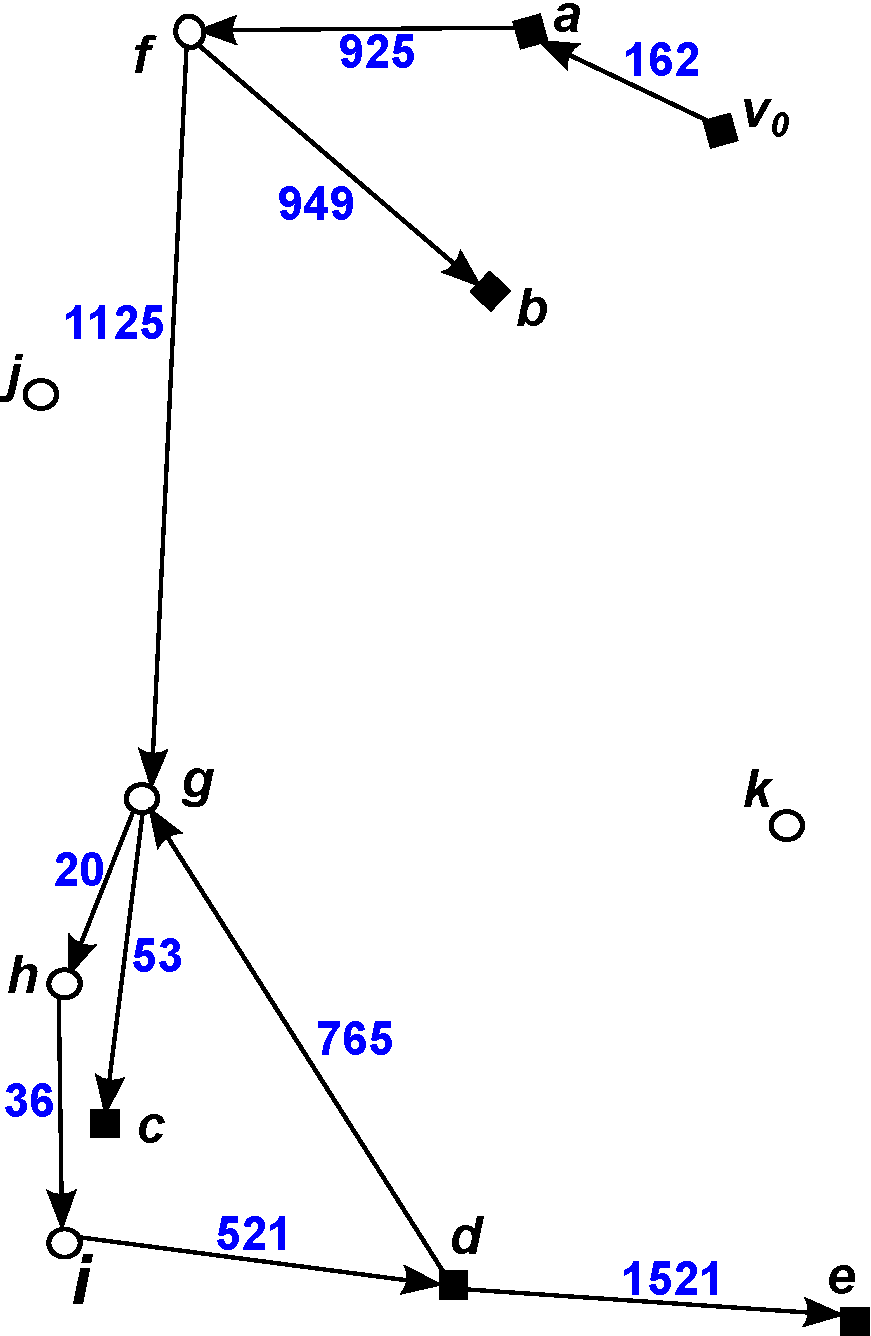
\includegraphics[width=\textwidth]{conBNec2}
        \caption{Solution obtained by F1 without constraint \ref{con:pf1:B} with objective value 25148 is not a Steiner tree.
		 The nodes are connected by arrows because the solution is a directed graph with a predefined source $s_0$.}
        \label{fig:Bpf2}
    \end{subfigure}
    \caption{An exemplary instance showing why constraint (\ref{con:pf1:B}) is necessary in F1.
		Blue numbers denote power requuirements of connection between nodes.
		For better legibility, the distances of the links are not proportional.} 
    \label{fig:BProof}
\end{figure}

%%%%%%%%%%%%%%%%%%%%%%%%%%%%%%%%%%%%%%%
%                                     %
%         Proposition 1               %
%                                     %
%%%%%%%%%%%%%%%%%%%%%%%%%%%%%%%%%%%%%%%
\begin{prop}
\label{prop:modelcorrect}
If $(F,g)$ satisfies (\ref{con:pf1:xfrel}) - (\ref{con:pf1:dim}) and (\ref{con:pf1:B})-(\ref{con:pf1:xi0=0}) then $G_{g}$ is a Steiner arborescence spanning $D$ rooted at $s_0$.
\end{prop}
 
\begin{proof}
The connectivity of $G_{g}$ as well as coverage of all nodes from $D$ is ensured by flow constraints (\ref{con:pf1:flow}) and relation (\ref{con:pf1:xfrel}).
The absence of both directed and undirected cycles is enforced by (\ref{con:pf1:B})-(\ref{con:pf1:xi0=0}).
As discussed above, these constraints together imply that no node has more than one entering arc.
In particular for a destination $i\in D_0$, by utilizing first (\ref{con:pf1:fitt=xit}), next (\ref{con:pf1:flow}) for $t=i$, and finally (\ref{con:pf1:noflowFromT}), we get
$$\sum_{j\in V_i}g_{ji}=\sum_{j\in V_i}F_{ji}^i = 1+\sum_{j\in V_i}F_{ij}^i=1.$$
%Solutions, where nodes from $V\setminus D$ are leaves are excluded due to (\ref{con:pf1:flowX}).
\qed
\end{proof}

\begin{prop}\label{prop:transX}
Assume $(F,\pi,g)$ satisfies (\ref{con:pf1:xfrel}) - (\ref{con:pf1:dim}) and  (\ref{con:pf1:B}) - (\ref{con:pf1:dimy}). Then
$$
g_{ij} - F^t_{ij}+F^t_{ji} = 
	\begin{cases}
		1, ~(i,j)~\text{is an arc on the path from~$t\in D_0$ in $G_{g}$} \\
		0, ~\text{otherwise.}
	\end{cases}
$$
\end{prop}
%
\begin{proof}
Let $T=(V_T,E_T)$ be a tree covering $D$ induced by $g$, and consider an edge $\{i,j\}\in E_T$ dividing $T$ into two subtrees $T_i$ and $T_j$ rooted in $i$ and $j$, respectively.
Assume without loss of generality that $t\in T_i$.
Either $s_0$ and $t$ are both in $T_i$, in which case none of the arcs $(i,j)$ and $(j,i)$ carries a flow to $t$, or $s_0$ belongs to $T_j$, and there is a flow from $s_0$ via $(j,i)$ towards $t$.
That is expressed in F-space as
$
g_{ij}(1-F^{t}_{ij})(1-F^{t}_{ji})+g_{ji}F^{t}_{ji}=g_{ij} - F^t_{ij}+F^t_{ji},
$
where the equality follows from (\ref{con:pf1:xfrel}).
\qed
\end{proof}

\begin{cor}
F1 is a correct formulation of Problem \ref{def:problem}.
\end{cor}

\subsubsection{Valid inequalities [F2]}

The same valid inequalities  leading to X2 are added to F1, resulting in the model denoted as F2.
Inequality (\ref{con:vi:Y1}) is added without any change.
The $x$-variable in (\ref{con:vi:sumYImpSumX}) has to be replaced by the equivalent expression from Prop. \ref{prop:transX}. 
Subsequent application of flow conservation (\ref{con:pf1:flow}) yields
%%%%%%%%%%%%%%%%%%%%%%%%%%%%%%%%%%%%%%%
%                                     %
%             MODEL F1VI              %
%            (4a) - (4m)              %
%                                     %
%%%%%%%%%%%%%%%%%%%%%%%%%%%%%%%%%%%%%%%
\begin{subequations}[resume]
\begin{flalign}
\label{con:vi:sumYImpSumXTrans} \sum\limits_{j\in V_i }\pi^{s}_{ij} & \geq \sum\limits_{j\in V_i}  g_{ji}  \quad\quad   i\in V\setminus D, s\in D. 
\end{flalign}
\end{subequations}
%
Further strengthening can be achieved by including 
\begin{subequations}[resume]
\begin{flalign}
\label{con:pf1:flowX}  \sum\limits_{\substack{ j\in V_i }}g_{ji}-\sum\limits_{\substack{j\in V_i}}g_{ij}    & \leq 0    \qquad\qquad			  i\in V\setminus D 
\end{flalign}
\end{subequations}
introduced in \cite{Polzin}, which is also analogous to (\ref{con:dd:extraCon}).
%This constraint is analogous to ($\ref{con:dd:extraCon})$, and is also obtained by applying (\ref{eq:tr:xijsB}) together with (\ref{con:pf1:flow}).

\subsubsection{Double flow extension [F3]}

Similarly to the extension X3 of X2 by $x$-variables, the model F2 can also be extended by variables with four node indices.
Analogously to $S$, let $\check{S}=\{\{s,t\}\subseteq D: s\neq t\}$ be the set of unordered pairs of destinations, and let $\check{S}_0=\{\{s,t\}\in S: s\neq s_0\neq t\}$.
 
The authors of \cite{Polzin} use variables
\newline\newline
$f^{st}_{ij}=
\begin{cases}
    1 & \text{if arc $(i,j) \in A$ lies on a path  from $s_0$ to both $s$ and $t$, $\{s,t\}\in \check{S}_0$},\\
    0 & \text{otherwise},
\end{cases}$
\newline\newline
which can also be regarded as a describtion of a common flow from $s_0$ to $s$ and $t$.
%describing a common flow from $s_0$ to $s$ and $t$.
%It is now possible to express variables $x^{st}_{ij}$ from $X2$ in the F3 space as 
%
%\begin{align}
%\label{eq:tr:fstij1}
%\begin{aligned}
%x^{st}_{ij}&=F^t_{ij}(1-f^{st}_{ij})+F^{s}_{ji}(1-f^{st}_{ji})= \\
%  	   &=  F^t_{ij}+F^s_{ji} - f^{st}_{ij} - f^{st}_{ji}\\
%x^{0t}_{ij}&=F^t_{ij}\\
%\end{aligned}
%&&
%\begin{aligned}
%\\
%(i,j)\in A, \{s,t\}\in S_0\\
%(i,j)\in A, t\in S_0.
%\end{aligned}
%\end{align}
%
This allows formulation of an extended model denoted as F3: 
%%%%%%%%%%%%%%%%%%%%%%%%%%%%%%%%%%%%%%%
%                                     %
%             MODEL F2                %
%     (4a) - (4m) and (5b) - (5f)     %
%                                     %
%%%%%%%%%%%%%%%%%%%%%%%%%%%%%%%%%%%%%%%
\begin{subequations}[resume]
\begin{align}
\notag\min & \sum\limits_{(i,j) \in A} \sum\limits_{s \in D} p_{ij} \pi^s_{ij}\\ \notag
\text{s.t.}& && \\
%(\ref{con:pf1:xfrel}) - (\ref{con:pf1:flowX}),& \notag \\
\notag(\ref{con:pf1:flow}) &- (\ref{con:pf1:flowX})\\
\label{con:pf2:flowHook} \sum\limits_{\substack{ j \in V_i }}f^{st}_{ji}-\sum\limits_{\substack{j\in V_i}}f^{st}_{ij} & \geq 
  \begin{cases}
    -1 & \{s,t\}\in \check{S_0}, i = 0, \\
    0  & \{s,t\}\in \check{S_0}, i\in V\setminus \{s_0\},
  \end{cases}  \\
\label{con:pf2:startInSource}  f^{st}_{ij} & \leq F^s_{ij} \quad \{s,t\}\in \check{S_0}, (i,j)\in A,\\
\label{con:pf2:stopInDest}  f^{st}_{ij} & \leq F^t_{ij} \quad \{s,t\}\in \check{S_0}, (i,j)\in A,\\
\label{con:pf2:stronger}  F^{s}_{ij}+F^{t}_{ij}-f^{st}_{ij} &\leq g_{ij} \quad \{s,t\}\in \check{S_0}, (i,j)\in A,\\ 
\label{con:pf2:sumFImpSumY} \sum\limits_{k\in V_j, p_{jk}\geq p_{ji}}F^{t}_{jk} + F^{s}_{kj} - f^{st}_{jk} - f^{st}_{kj} & \leq \sum\limits_{k\in V_j, p_{jk}\geq p_{ji}}  \pi^{s}_{jk} \quad i,j\in V,\{s,t\}\in \check{S_0},\\
\label{con:pf2:sumFImpSumY2} \sum\limits_{k\in V_j, p_{jk}\geq p_{ji}}F^{t}_{jk} & \leq \sum\limits_{k\in V_j, p_{jk}\geq p_{ji}}  \pi^{0}_{jk} \quad i,j\in V, t\in D_0,\\
\label{con:pf2:dim} f&\in\{0,1\}^{A\times \check{S}}.
\end{align}~
\end{subequations}

By (\ref{con:pf2:flowHook}) is ensured that the common flow is non-increasing.
The inequalities (\ref{con:pf2:stronger}) replace a weaker (\ref{con:pf1:xfrel}).
Finally, (\ref{con:pf2:sumFImpSumY}) - (\ref{con:pf2:sumFImpSumY2}) is a valid inequality (\ref{con:vi:sumFImpSumY}) implied by the following

\begin{prop}\label{prop:transX}
Assume $(F,f,\pi,g)$ satisfies (\ref{con:pf1:flow}) - (\ref{con:pf2:stronger}). Then
$$
F^t_{ij}+F^s_{ji}-f^{st}_{ij}-f^{st}_{ji} = 
	\begin{cases}
		1, ~(i,j)~\text{is an arc on the path from~$s$ to $t$ in $G_{g}$} \\
		0, ~\text{otherwise.}
	\end{cases}
$$
\end{prop}
%
\begin{proof}

Let $T=(V_T,E_T)$ be a tree covering $D$, and consider an edge $\{i,j\}\in E_T$ dividing $T$ into two subtrees $T_i$ and $T_j$ rooted in $i$ and $j$, respectively.
If the arc $(i,j)$ carries flow from $s\in D$ to $t\in D$, then $s$ and $t$ must lie in different subtrees.
Node $s_0$ lies either in $T_i$ or $T_j$.
%as depicted in Fig. \ref{fig:transf_a} and Fig. \ref{fig:transf_b}, respectively.
These two cases are captured by the first equality in (\ref{eq:tr:fstij}).
If both $s_0$ and $s$ lie in $T_i$, then $f_{ij}^t=1$.
Similarly, if $s_0$ and $t$ lie in $T_j$, then $f_{ji}^s=1$.
The expressions in parentheses prevent $s$ and $t$ belonging to the same subtree.
Using the implications $\check{f^{st}_{ij}}=1\Rightarrow f_{ij}^t=1$ and $\check{f^{st}_{ji}}=1\Rightarrow f_{ji}^s=1$ that follow from the interpretation of variables, we justify the second equality expressing this relation linearly.
\begin{subequations}
\begin{align}
\notag\label{eq:tr:fstij}f^{st}_{ij}&=f^t_{ij}(1-\check{f}^{st}_{ij})+f^{s}_{ji}(1-\check{f}^{st}_{ji})= \\
  &=  f^t_{ij}+f^s_{ji} - \check{f}^{st}_{ij} - \check{f}^{st}_{ji}& (i,j)\in A, \{s,t\}\in S_0\\
\notag\label{eq:tr:xijj}x^s_{ij}&=x_{ij}(1-f^{s}_{ij})(1-f^{s}_{ji})+x_{ji}f^{s}_{ji}=\\
  &= x_{ij}-f^s_{ij} + f^{s}_{ji} & (i,j)\in A, s\in D_0\\
\label{eq:tr:zij}z_{ij}&=x_{ij}+x_{ji}& \{i,j\}\in E
\end{align}
\end{subequations}
\qed
\end{proof}
%%%%%%%%%%%%%%%%%%%%%%%%%%%%%%%%%%%%%%%%%%%%%%%%%%%%%%%%%%%
%	Additional VI following from implicit symmetry 5  %
%%%%%%%%%%%%%%%%%%%%%%%%%%%%%%%%%%%%%%%%%%%%%%%%%%%%%%%%%%%
%It follows from the domain of $f$, that 
%\begin{equation}
%\label{eq:fhooksym}f_{ij}^{st}=f_{ij}^{ts},
%\end{equation}
%because $S_0$ consists of unordered pairs. 
%By the implicit assumption of (\ref{eq:fhooksym}) in SMT-F2, it is possible to infer additional valid inequalities for SMT. We can also write
%\begin{align*}
%f^{st}_{ij}+f^{st}_{ji}=f^{ts}_{ij}+f^{ts}_{ji} &\Rightarrow F^t_{ij}+F^s_{ji}-x^{st}_{ij}=F^s_{ij}+F^t_{ji}-x^{ts}_{ij}\Rightarrow \\ & \Rightarrow x^{0t}_{ij}+x^{0s}_{ji}-x^{st}_{ij}=x^{0s}_{ij}+x^{0t}_{ji}-x^{ts}_{ij}.
%\end{align*}
%The first and second implication follow from the transformation (\ref{eq:tr:fstij}) and (\ref{eq:tr:fijt2}), respectively. The last equality consists of only variables from SMT-X2  space, and so the valid inequality
%\begin{equation*}
%x^{ut}_{ij}+x^{us}_{ji}+x^{ts}_{ij}=x^{us}_{ij}+x^{ut}_{ji}+x^{st}_{ij} \quad\quad (u,t),(u,s),(s,t),(t,s)\in S_0, i,j\in V
%\end{equation*}
%can be added to  SMT-X2. All the occurances of $s_0$ were replaced by a general destination $u\in D$, because $s_0$ does not have any special role in SMT-X2.

%\subsubsection{Valid inequalities [F2VI]}

%To complete the listing of models, we state the model F2VI created by adding transformed valid inequalities (\ref{con:vi:f2dest})-(\ref{con:vi:sumFImpSumY}) to F2.


